% Propósito: distinguir presión de fuerza y mostrar cómo una diferencia de
% presión uniforme sobre un área produce una fuerza neta.
% Origen: Delta p=p_1-p_2 y F_pres=Delta p A, ecuación
% \eqref{eq:u2-presion-fuerza}. Esquema cualitativo, no a escala.
% Descripción accesible: una superficie vertical de área A separa dos regiones.
% La presión p_1 del lado izquierdo empuja hacia la derecha y la presión p_2
% del lado derecho empuja hacia la izquierda. Cuando p_1 es mayor que p_2, la
% fuerza neta F_pres apunta hacia la derecha.
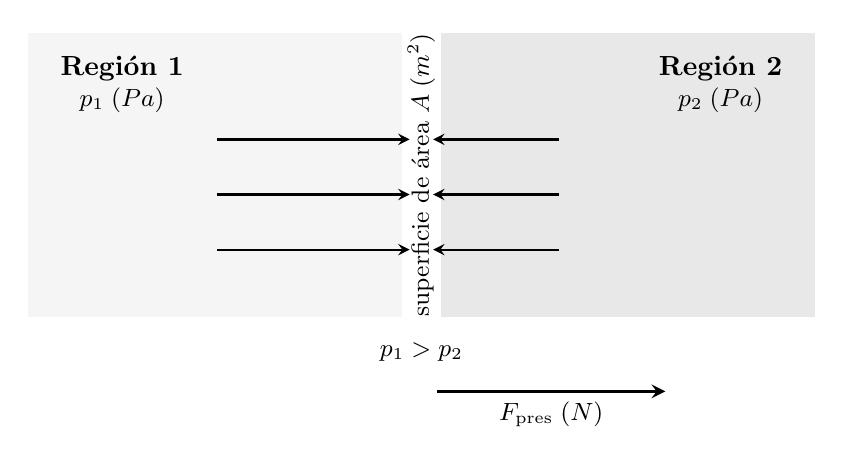
\begin{tikzpicture}[font=\small,>=stealth,x=1cm,y=1cm]
    \fill[black!4] (-5,-1.8) rectangle (0,1.8);
    \fill[black!9] (0,-1.8) rectangle (5,1.8);

    \draw[very thick] (0,-1.8) -- (0,1.8);
    \node[rotate=90,fill=white,inner sep=2pt] at (0,0)
        {superficie de área \(A\;(\text{m}^{2})\)};

    \node[font=\bfseries] at (-3.8,1.35) {Región 1};
    \node at (-3.8,0.95) {\(p_1\;(\text{Pa})\)};
    \node[font=\bfseries] at (3.8,1.35) {Región 2};
    \node at (3.8,0.95) {\(p_2\;(\text{Pa})\)};

    \foreach \y in {-0.95,-0.25,0.45}{
        \draw[->,thick] (-2.6,\y) -- (-0.15,\y);
        \draw[->,thick] (1.75,\y) -- (0.15,\y);
    }

    \node at (0,-2.25) {\(p_1>p_2\)};
    \draw[->,very thick] (0.2,-2.75) -- (3.1,-2.75)
        node[midway,below] {\(F_\mathrm{pres}\;(\text{N})\)};
\end{tikzpicture}
